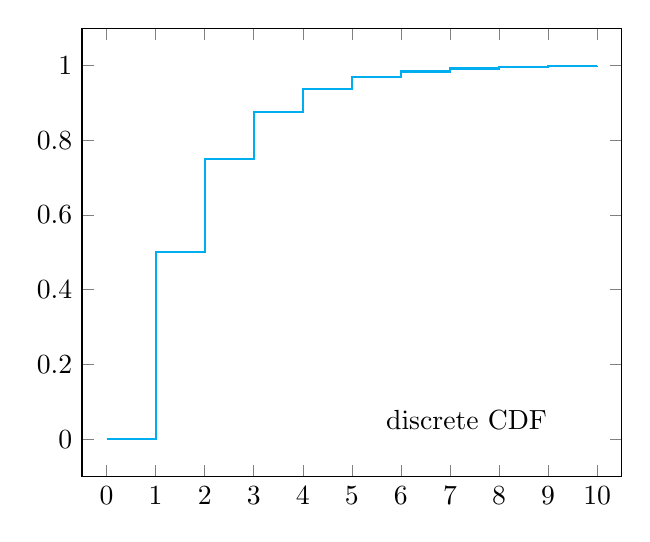
\begin{tikzpicture}
  \begin{axis}[
      axis lines=box,
      xtick={0,1,...,10},
      ytick={0,0.2,...,1},
      ymin=-0.1, ymax=1.1,
      xmin=-0.5, xmax=10.5,
      every axis x label/.style={at={(ticklabel* cs:1)}, anchor=north},
      every axis y label/.style={at={(ticklabel* cs:1)}, anchor=east},
  ]
      % Plot the stepwise CDF
      \addplot[
          thick,
          cyan,
          const plot
      ] coordinates {
          (0, 0)
          (1, 0.5)
          (2, 0.75)
          (3, 0.875)
          (4, 0.9375)
          (5, 0.96875)
          (6, 0.984375)
          (7, 0.9921875)
          (8, 0.99609375)
          (9, 0.998046875)
          (10, 0.999023437)
      };

      % Add "discrete CDF" label
      \node[anchor=south west] at (axis cs:5.5,0) {discrete CDF};
  \end{axis}
  \end{tikzpicture}